\documentclass[11pt,reqno,final]{amsart}
\usepackage[font=small,margin=10pt,labelfont={bf},labelsep={space}]{caption}
\usepackage{subfig}
\usepackage{wrapfig}
\usepackage{amsmath, amssymb, epsfig}
\usepackage[scaled]{helvet} % I like Helvetica for sf
\usepackage{fourier}
\usepackage{bm}
\usepackage{color}
\usepackage{fullpage} 	% Fullpage package
%\usepackage{cite}
%\usepackage{citesort}
\newcommand{\notate}[1]{\textcolor{red}{\textbf{[#1]}}}
%\input{macros}


\newcommand{\tasos}{\text{TASOS}}
%Results
%Shortcuts
\newcommand{\hide}[1]{}
\newcommand{\R}{\mathbb{R}}
\newcommand{\E}{\mathbb{E}}
\newcommand{\N}{\mathbb{N}}
\newcommand{\Z}{\mathbb{Z}}

\newcommand{\x}{\mathbf{x}}
\newcommand{\y}{\mathbf{y}}
\newcommand{\z}{\mathbf{z}}
%\newcommand{\A}{\mathbf{A}}
\newcommand{\bi}{\mathbf{b}}
\newcommand{\ro}{\mathbf{r}}
\newcommand{\w}{\mathbf{w}}
\newcommand{\zero}{\mathbf{0}}
\newcommand{\ep}{\epsilon}
\newcommand{\de}{\delta}
\newcommand{\defby}{\overset{\mathrm{\scriptscriptstyle{def}}}{=}}
\newcommand{\bigO}{\mathrm{O}}
\DeclareMathOperator*{\argmin}{arg min}
\DeclareMathOperator*{\argmax}{arg max}
%************************************
%************************************
% The macros below are due to Tassos Zouzias
%************************************
%************************************

\newcommand{\eps}{\varepsilon}


\newcommand{\Prob}[1]{\ensuremath{\mathbb{P}\left(#1\right)}}

\newcommand{\OO}{\mathcal{O}}
\newcommand{\vol}[1]{\text{vol}(#1)}
\newcommand{\tr}{\rm{Tr}}
\newcommand{\RR}{\mathbb{R}}
\newcommand{\NN}{\mathbb{N}}
\newcommand{\reals}{\mathbb{R}}


\newcommand{\e}{\ensuremath{{\rm e}}}
\DeclareMathOperator{\EE}{\mathbb{E}}
% Variance
\newcommand{\var}[1]{\ensuremath{\mathrm{Var}(#1)}}
% Pseudo-inverse of a matrix
\newcommand{\pinv}[1]{ {#1}^\dagger}
\newcommand{\norm}[1]{\ensuremath{\left\|#1\right\|_2}}
\newcommand{\pnorm}[1]{\ensuremath{\left\|#1\right\|_p}}
\newcommand{\qnorm}[1]{\ensuremath{\left\|#1\right\|_q}}
\newcommand{\infnorm}[1]{\ensuremath{\left\|#1\right\|_\infty}}
\newcommand{\onenorm}[1]{\ensuremath{\left\|#1\right\|_1}}
\newcommand{\frobnorm}[1]{\ensuremath{\left\|#1\right\|_{\text{\rm F}}}}
% Stable rank of a matrix
\newcommand{\sr}[1]{\ensuremath{\mathrm{\textbf{\footnotesize sr}}\left(#1\right)}}
% Trace of a matrix.
\newcommand{\trace}[1]{\ensuremath{\mathrm{\textbf{tr}}\left(#1\right)}}
%\DeclareMathOperator{\trace}{trace}
% Rank of a matrix
\newcommand{\rank}[1]{\ensuremath{\mathrm{\textbf{{\footnotesize rank}}}\left(#1\right)}}
% Kernel of a matrix
%\newcommand{\ker}[1]{\ensuremath{\mathrm{\textbf{ker}}\left(#1\right)}}
% Image of a matrix
\newcommand{\im}[1]{\ensuremath{\mathrm{\textbf{Im}}\left(#1\right)}}

% Condition number of a matrix
\newcommand{\cond}[1]{\ensuremath{\mathrm{\text{cond}}\left(#1\right)}}

\newcommand{\expm}[1]{\ensuremath{\mathrm{\textbf{\footnotesize exp}}\left[#1\right]}}
\newcommand{\coshm}[1]{\ensuremath{\mathrm{\textbf{\footnotesize cosh}}\left[#1\right]}}
\newcommand{\detm}[1]{\ensuremath{\mathrm{\textbf{det}}\left(#1\right)}}
\newcommand{\sign}[1]{\ensuremath{\mathrm{\textbf{sign}}\left(#1\right)}}


% # of non-zero entries of a matrix
\newcommand{\nnz}[1]{\ensuremath{\mathrm{\textbf{\footnotesize nnz}}\left(#1\right)}}

% Diagonal Matrix
\newcommand{\diag}[1]{\ensuremath{\mathrm{\textbf{diag}}\left(#1\right)}}
% Polylog(n)
\newcommand{\polylog}[1]{\ensuremath{\mathrm{polylog}\left(#1\right)}}

\newcommand{\old}{\text{old}}
\newcommand{\new}{\text{new}}
\newcommand{\ravg}{\text{R}_{\text{avg}}}
\newcommand{\cavg}{\text{C}_{\text{avg}}}
%\newcommand{\cavg}[1]{\text{C}_{\text{avg}}(#1)}


%%% Vector and matrix operators

\newcommand{\vct}[1]{\bm{#1}}
\newcommand{\mtx}[1]{\bm{#1}}

\newcommand{\ip}[2]{\left\langle {#1},\ {#2} \right\rangle}
\newcommand{\mip}[2]{ {#1}\bullet {#2}}

\newcommand{\ignore}[1]{}

\newcommand{\Id}{\mathbf{I}}
\newcommand{\J}{\mathbf{J}}
\newcommand{\onemtx}{\bm{1}}
%\newcommand{\zeromtx}{\bm{0}}
\newcommand{\zeromtx}{\mathbf{0}}




%%%%%%%%%%%%%%%%%%%%%%%%%%%%%%%%%%%%%
\newcommand{\mat}[1]{ {\ensuremath{\mtx{#1} }}}
%%%%%%%%%%%%%%%%%%%%%%%%%%%%%%%%%%%%%

\def\gammab{{\bm{\gamma}}}
\def\kappab{{\bm{\kappa}}}
\def\sig{{\bm{\Sigma}}}
\def\sigplus{{\bm{\Sigma}^{+}}}
\def\siginv{{\bm{\Sigma}^{-1}}}
\def\bet{{\bm{\beta}}}
\def\one{{\bm{1}}}
\def\exp{\hbox{\rm exp}}
\def\col{\hbox{\rm col}}
\def\ker{\hbox{\rm ker}}
\def\ahat{{\hat\a}}
\def\p{{\mathbf p}}
\def\e{{\mathbf e}}
\def\q{{\mathbf q}}
\def\rb{{\mathbf r}}
\def\s{{\mathbf s}}
\def\u{{\mathbf u}}
\def\v{{\mathbf v}}
\def\d{{\mathbf \delta}}
\def\xhat{{\hat\x}}
\def\yhat{{\hat\y}}
\def\A{\matA}
\def\B{\matB}
\def\C{\matC}
\def\Ahat{\hat\matA}
\def\Atilde{\tilde\matA}
\def\Btilde{\tilde\matB}
\def\Stilde{\tilde\matS}
\def\Utilde{\tilde\matU}
\def\Vtilde{\tilde\matV}
\def\G{{\cl G}}
\def\hset{{\cl H}}
\def\Q{{\bm{Q}}}
\def\U{{\bm{U}}}
\def\V{{\bm{V}}}
\def\win{\hat{\w}}
\def\wopt{\w^*}
\def\matAhat{\hat\mat{A}}
\def\matA{\mat{A}}
\def\matB{\mat{B}}
\def\matC{\mat{C}}
\def\matD{\mat{D}}
\def\matE{\mat{E}}
\def\matH{\mat{H}}
\def\matI{\mat{I}}
\def\matM{\mat{M}}
\def\matP{\mat{P}}
\def\matQ{\mat{Q}}
\def\matR{\mat{R}}
\def\matL{\mat{L}}

\def\matS{\mat{S}}
\def\matT{\mat{T}}
\def\matU{\mat{U}}
\def\matV{\mat{V}}
\def\matW{\mat{W}}
\def\matX{\mat{X}}
\def\matY{\mat{Y}}
\def\matZ{\mat{Z}}
\def\matSig{\mat{\Sigma}}
\def\matOmega{\mat{\Omega}}
\def\matGam{\mat{\Gamma}}
\def\matTheta{\mat{\Theta}}
\def\w{{\mathbf{w}}}
\def\ein{{\cl E_{\text{\rm in}}}}
\def\eout{{\cl E}}
\def\scl{{\textsc{l}}}
\def\scu{{\textsc{u}}}
\def\phiu{{\overline{\phi}}}
\def\psiu{{\overline{\psi}}}
\def\phil{{\underbar{\math{\phi}}}}
\newcommand\remove[1]{}


\newcommand{\vecb}{{\vct{b} }}
\newcommand{\bc}{{\vecb_{\mathcal{R}(\matA)^\bot } }}
\newcommand{\br}{{\vecb_{\mathcal{R}(\matA) } }}

% Least squares solution of Ax = b
\def\xls{\x_{\text{\tiny LS}}}

% For rows and columns of a matrix A
\newcommand{\ar}[1]{ \matA^{(#1)}}
\newcommand{\ac}[1]{ \matA_{(#1)}}

\newcommand{\colspan}[1]{\mathcal{R}(#1)}

\usepackage{palatino}

%---------------------Listings--------------------%
\usepackage{listings}
\usepackage{color}
\definecolor{dkgreen}{rgb}{0,0.6,0}
\definecolor{gray}{rgb}{0.5,0.5,0.5}
\definecolor{mauve}{rgb}{0.58,0,0.82}
\lstset{ %
  language=Octave,                % the language of the code
  basicstyle=\footnotesize,           % the size of the fonts that are used for the code
  numbers=left,                   % where to put the line-numbers
  numberstyle=\tiny\color{gray},  % the style that is used for the line-numbers
  stepnumber=2,                   % the step between two line-numbers. If it's 1, each line
                                  % will be numbered
  numbersep=5pt,                  % how far the line-numbers are from the code
  backgroundcolor=\color{white},      % choose the background color. You must add \usepackage{color}
  showspaces=false,               % show spaces adding particular underscores
  showstringspaces=false,         % underline spaces within strings
  showtabs=false,                 % show tabs within strings adding particular underscores
  frame=single,                   % adds a frame around the code
  rulecolor=\color{black},        % if not set, the frame-color may be changed on line-breaks within not-black text (e.g. commens (green here))
  tabsize=2,                      % sets default tabsize to 2 spaces
  captionpos=b,                   % sets the caption-position to bottom
  breaklines=true,                % sets automatic line breaking
  breakatwhitespace=false,        % sets if automatic breaks should only happen at whitespace
  title=\lstname,                   % show the filename of files included with \lstinputlisting;
                                  % also try caption instead of title
  keywordstyle=\color{blue},          % keyword style
  commentstyle=\color{dkgreen},       % comment style
  stringstyle=\color{mauve},         % string literal style
  escapeinside={\%*}{*)},            % if you want to add LaTeX within your code
  morekeywords={*,...}               % if you want to add more keywords to the set
}
%-------------------------------------------------%

%%%%%%%%%%%%%%%%%%%%%%%%%%%%%%%%%%%%%%%%%%%%%%%%%%%%%%%%%%%%%%%%%%%
%%%%%%%%%%%%%%%%%%%%%%%%%%%%%%%%%%%%%%%%%%%%%%%%%%%%%%%%%%%%%%%%%%%
%%%%%%%%%%%%%%%%%%%%%%%%%%%%%%%%%%%%%%%%%%%%%%%%%%%%%%%%%%%%%%%%%%%
\usepackage{hyperref}

\usepackage[T1]{fontenc}
\usepackage[utf8]{inputenc}
\usepackage{tabularx,ragged2e,booktabs,caption}

% Place this after the backref command
\usepackage{algorithmicx}
\usepackage[ruled]{algorithm}
\usepackage{algpseudocode}

\newcommand{\floor}[1]{\lfloor #1 \rfloor}
\newtheorem{definition}{Definition}
\newtheorem{theorem}{Theorem}
\newtheorem{proposition}[theorem]{Proposition}
\newtheorem{lemma}[theorem]{Lemma}
\newtheorem{corollary}[theorem]{Corollary}
\newtheorem{question}{Question}
\newtheorem{claim}[theorem]{Claim}
\newtheorem{conjecture}[theorem]{Conjecture}
\newtheorem{observation}[theorem]{Observation}
\newtheorem{fact}[theorem]{Fact}
\newtheorem{example}{Example}
%\newtheorem{algorithm}{Algorithm}
\newtheorem{assumption}[theorem]{Assumption}
\newtheorem{remark}{Remark}
\newtheorem{problem}{Problem}

%-------------------------------------------------%


%%%%%%%%%%%%%%
% Document
%%%%%%%%%%%%%%


\title{Implied Volatility Surface and Model of VIX}
\author{Ran Zhao}
\thanks{}
\begin{document}

%%%%%%%%%%%%%%%%%%%%%%%%%%%%%%%%%%%%%%%%%%%%%%%%%%
%%%%%%%%%%%%%%%%%%%%%%%%%%%%%%%%%%%%%%%%%%%%%%%%%%
\begin{abstract}
In this paper, we first back out the Black-Scholes implied volatility based on real dated VIX options. An obvious observation is that the VIX implied volatilities are upward-sloping, in opposite to the implied volatility skew for SPX index options. Also there are at least two factors that drive the dynamic of VIX implied volatilities, since the volatility smile varies with short-term and long-term VIX levels. Then we derive that any twice-differentiable payoff at time $T$ may be statically hedged using a portfolio of European options expiring at time $T$. And $VIX^2$ is the fair strike of a variance swap, and the fair value of $VIX^2$ can be calculated from the strip of European options. Finally, we propose double stochastic volatility model with diffusion underlying dynamic for jointly SPX and VIX options modeling.
\end{abstract}

\maketitle
%%%%%%%%%%%%%%%%%%%%%%%%%%%%%%%%%%%%%%%%%%%%%%%%%%%
%%%%%%%%%%%%%%%%%%%%%%%%%%%%%%%%%%%%%%%%%%%%%%%%%%%
%
%
%
\section{Introduction}
Black~\cite{Black76} first introduced the European futures options pricing based on Black-Scholes framework~\cite{BS73}. The common assumption for the process followed by future price $F$ in risk-neutral framework is
\begin{equation}
dF=\sigma F dW,
\end{equation}

where $\sigma$ is a constant and $W$ is the Wiener process. Similar to a non-dividend-paying stock, the differential equation satisfied by a derivative dependent on a futures price is
$$
\frac{\partial f}{\partial t} + \frac{1}{2} \frac{\partial^2 f}{\partial F^2} \sigma^2 F^2 = rf.
$$

Then the European call price $c$ and the European put price $p$ for the futures option are given by following equations,
\begin{eqnarray}
c &=& e^{-rT}[F_0 N(d_1) - KN(d_2)],  \label{eqn::future_bs} \\
p &=& e^{-rT}[K N(-d_2) - F_0 N(-d_1)], \notag \\
\end{eqnarray}

where
\begin{eqnarray*}
d_1 &=& \frac{\log(F_0/K) + \sigma^2T/2}{\sigma\sqrt{T}}, \\
d_2 &=& \frac{\log(F_0/K) - \sigma^2T/2}{\sigma\sqrt{T}} = d_1 -\sigma\sqrt{T}. \\
\end{eqnarray*}

Following the Black-Scholes framework, more recent researches come up with stochastic volatility (SV) model~\cite{Heston93,Bates96,DPS00}, where the volatility surface (w.r.t. different terms and strikes) are fitted better to the empirical observations. The SV modelings are motivated by the intermittency and clustering feature of volatility from underlying dynamics. A common stochastic volatility process satisfies the SDE:
\begin{equation*}
dS_t = \mu_t S_t dt + \sqrt{v_t} S_t dW_1, \\
dv_t = \alpha(S_t,v_t,t)dt + \eta\beta(S_t,v_t,t)\sqrt{v_t} dW_2,
\end{equation*}
where $\mathbb{E}[dW_1 dW_2]=\rho dt$. $\mu_t$ is the (deterministic) instantaneous drift of stock price returns, $\eta$ is the volatility of volatility and $\rho$ is the correlation between random stock price returns and changes in $v_t$. $W1$ and $W_2$ are Wiener processes.

The volatility drift and vol of vol term are in most generic functional forms and can determine by time ($t$), instantaneous volatility level ($v_t$) and the spot price ($S_t$). Note that the SV setup ensures the standard time-dependent volatility version of the Black-Scholes formula may be retrieved in the limit $\eta \rightarrow 0$.

Particularly, S\&P500 index returns, shown in Figure~\ref{plot_spx}, reinforce the stochastic volatility and volatility mean-reverting characteristics. More importantly, the ``volatility'' of the S\&P500 index is tradable. The VIX index represents the volatility of SPX in a precise way, and CBOE has listed futures on VIX index since 2004 and VIX option in 2006.

\begin{figure}[H]
  \centering
  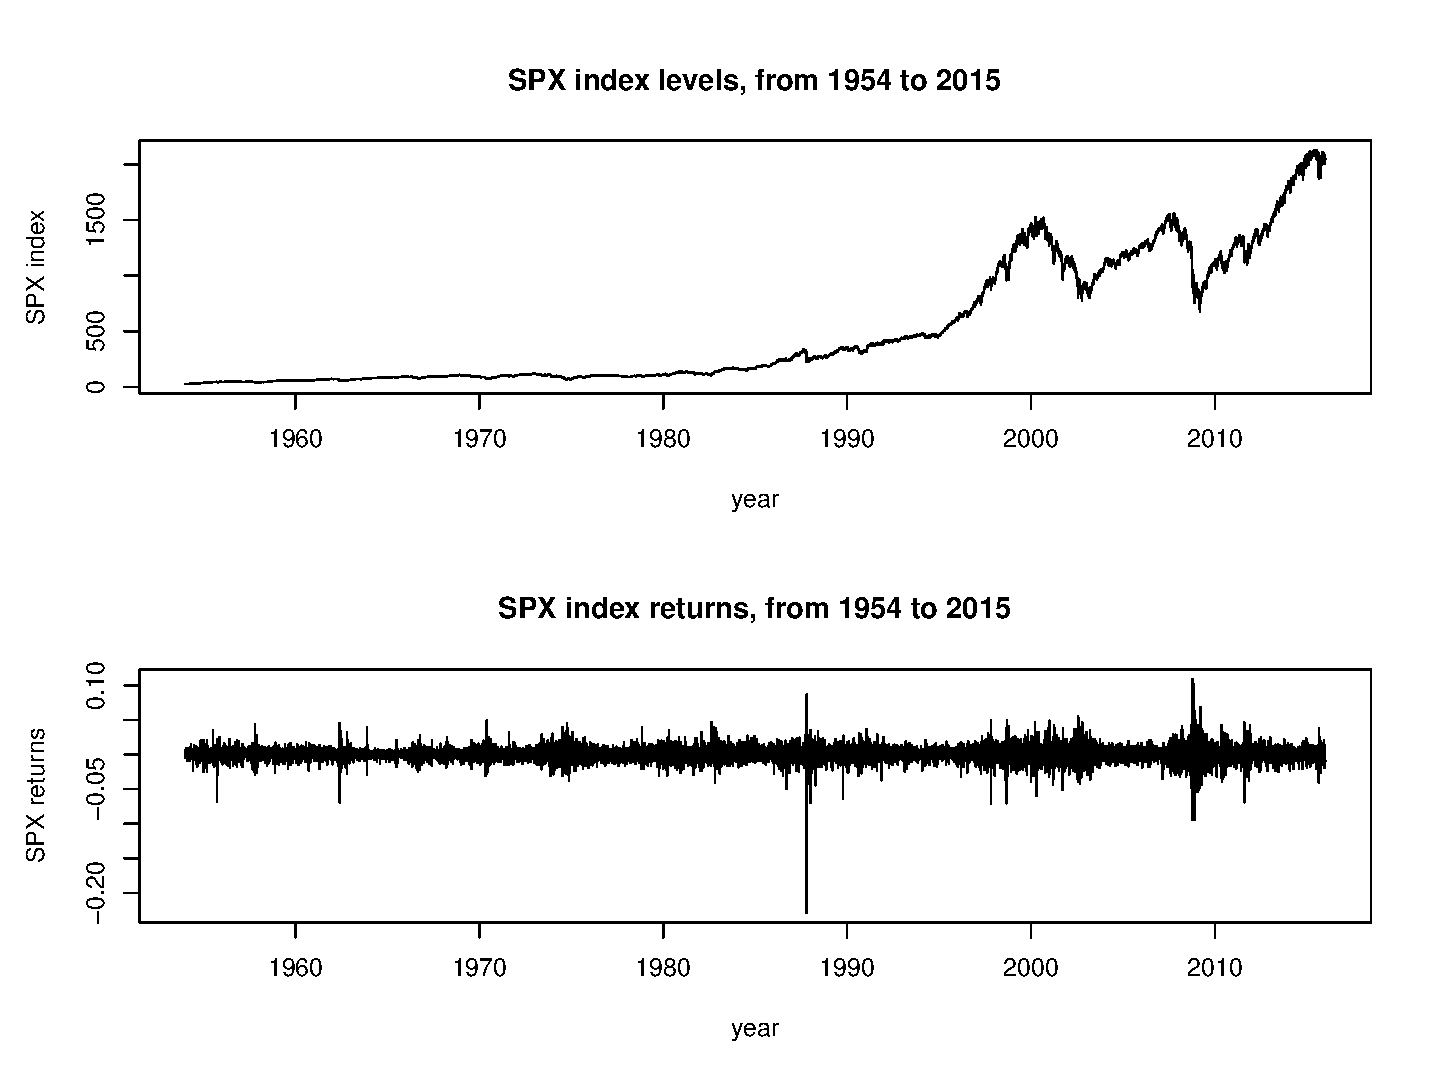
\includegraphics[scale=0.6]{spx_index_return.eps}
  \caption{The SPX index levels and return on daily basis. Time period is from 1954 to 2015.}\label{plot_spx}
\end{figure}

The rest of the paper lays out as following: Section~\ref{sec::vix_smile} presents the observations and findings on implied volatility from VIX options. Section~\ref{sec::vix_model} conjectures a two-factor VIX model and discusses the joint VIX model with SPX dynamics.

\bigskip

\section{VIX Implied Volatility} \label{sec::vix_smile}
The option data from OptionMetrics contains daily standardized VIX option bid/offer price, Delta of the option and other information including expiration and strike. The forward price, here the underlying future price, is interpolated from OptionMetrics' standard volatility surface using log-linear interpolation. The reasoning of selecting log-linear interpolation is that the future price is positively correlated with discount factor, and we assume a flat-forward interpolation keeps most of properties from term structure. The zero yield curve is also from OptionMetrics database.

\begin{figure}
  \centering
  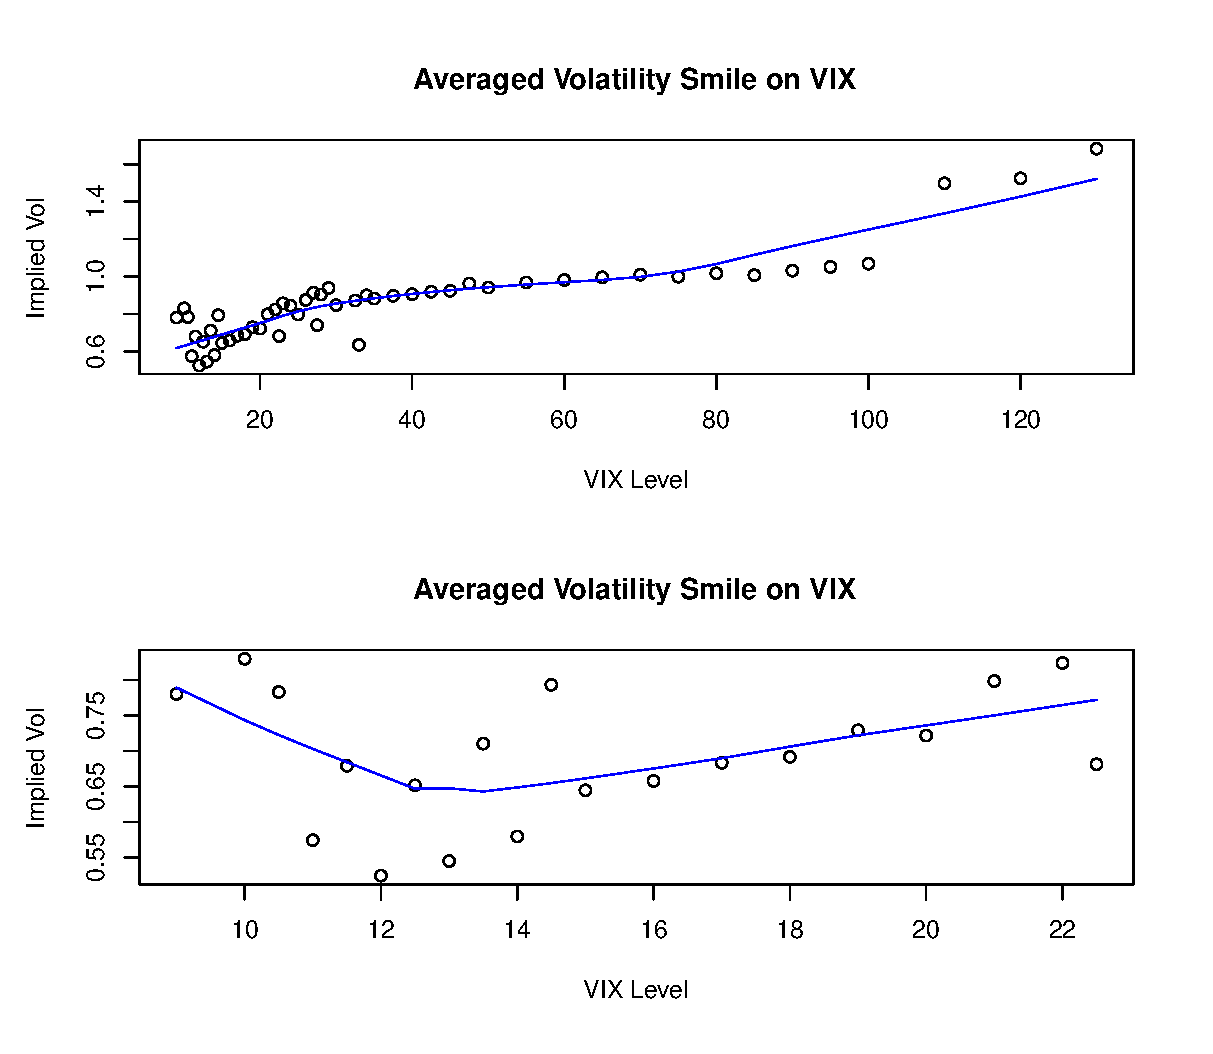
\includegraphics[scale=0.6]{avg_vix.eps}
  \caption{The averaged VIX option implied volatility over different terms. The graph plots the implied volatility dynamic on various strikes. The blue line is the fitted implied volatility smile by lowess regression. The graph on the top has strikes (of VIX) from 5 to 130. The graph on the bottom has strikes from 5 to 22.}\label{avg_vix}
\end{figure}

The VIX future has multiplier of 1000, so the strike price of options are in magnitude of 1000 times VIX. To back-out the implied volatility of VIX options, we use the Black model as specified in~\ref{eqn::future_bs}. The market premium is calculated from the average of best bid and best offer price. The underlying future price is interpolated log-linearly from standard option volatility, and the interest rate is interpolated linearly from the term structure of zero yield.

According call-put parity, the implied volatility from call option and put option with same strike will be the same. Figure~\ref{avg_vix} plots the averaged implied volatility over the terms. The graph on the top shows the implied volatility dynamics of VIX option with strike price ranging from 5\% to 130\%. Unlike the volatility skew shape as in equity option, the VIX option has higher implied vol (SPX's vol of vol). The strike-zoom-in graph on the bottom from Figure~\ref{avg_vix} show the volatility smile at relatively low VIX strike levels, ranging from 5\% to 23\%.

Figure~\ref{four_vix} separates the average on implied volatility when the short term and long term are high/low respectively. From the graphs, it is obvious that the implied volatility levels have different shapes, in terms of both magnitude and the slope. That is, the implied volatility smile of VIX options are not only driven by the VIX level, but also term structure and skew. Therefore, empirical observations conflict one-factor stochastic volatility model, which captures only the level of volatility but not sufficient to fit term structure additionally.

Then the idea of two-factor stochastic volatility modeling becomes natural. In Section~\ref{sec::vix_model}, we will discuss the rationale of the double-stochastic-variance (DSV) model.

\begin{figure}
  \centering
  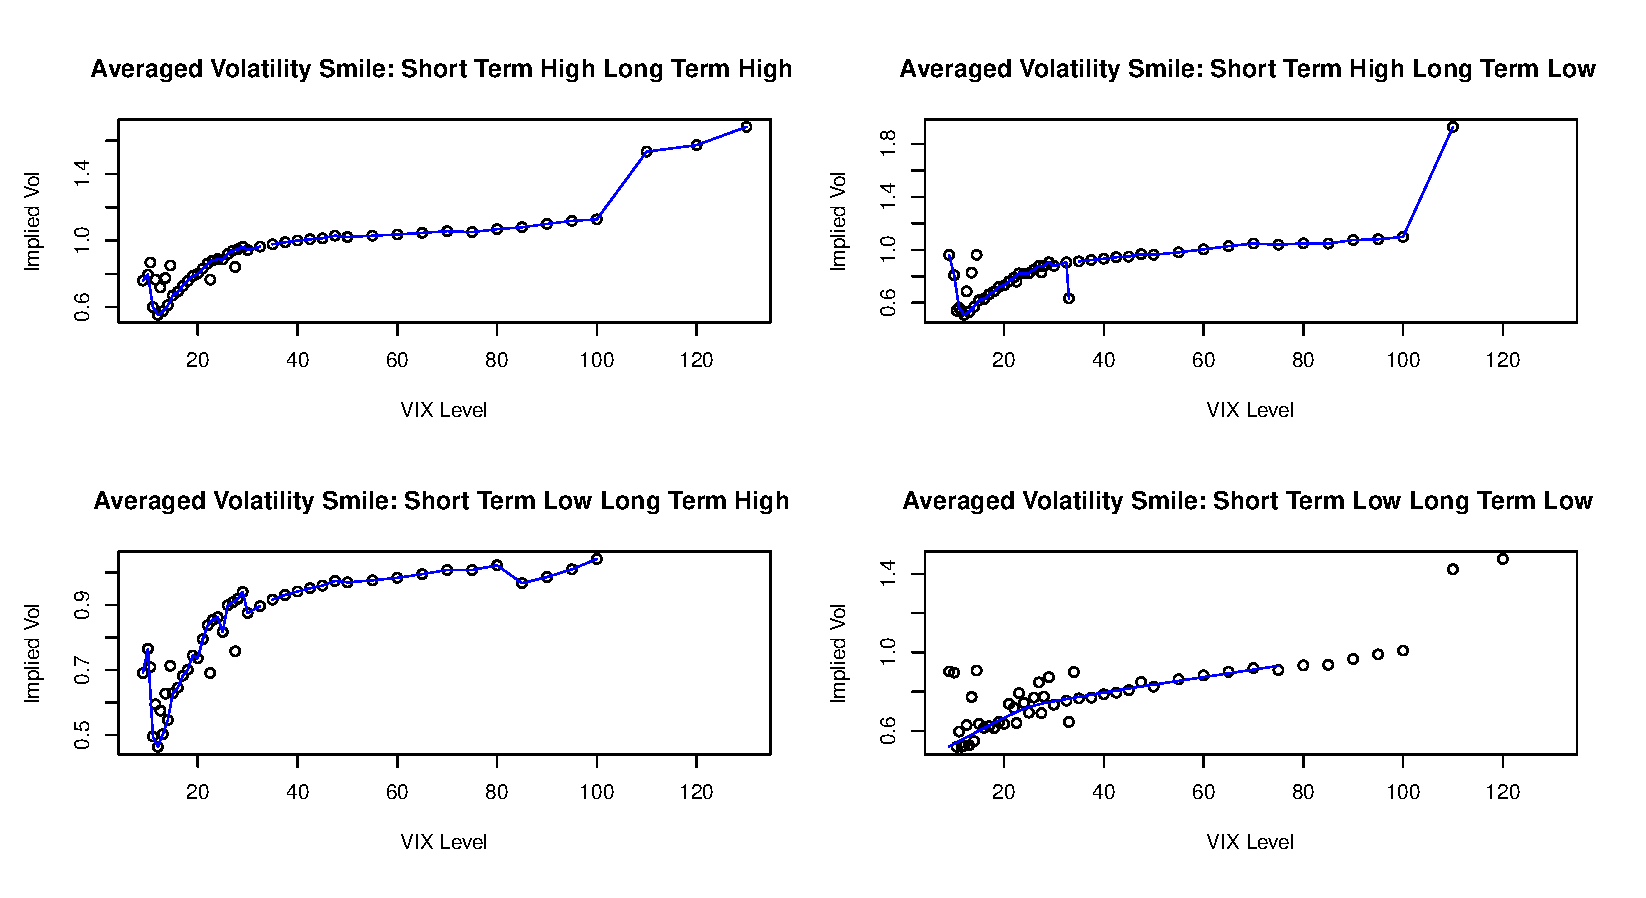
\includegraphics[scale=0.6]{four_vix.eps}
  \caption{The averaged VIX option implied volatility over different terms, when the short/long term implied volatilities are high/low. Four graphs display the combination of the short- and long-term VIX. Each graph plots the implied volatility dynamic on various strikes.}\label{four_vix}
\end{figure}


\bigskip


\section{Modeling VIX and SPX Jointly} \label{sec::vix_model}
Before proceeding to the conjecture of the VIX model, we firstly show that VIX represents the volatility of SPX in a precise way. Therefore one can model VIX using variance swap instead of the implied volatilities. And also the relationship between the prices of options on SPX and options on VIX can be established. In particular, the fair values of the variance swaps can be expressed in terms of the market prices of European options, which provides an model-independent way of linking SPX and VIX.

Assume there are European options with all possible strikes $K$ and maturity are traded on the market, then any twice-differentiable payoff at time $T$ may be statically hedged using a portfolio of European options expiring at time $T$. To prove this, consider the value of a claim with payoff $g(S_T)$ at time $T$ as
\begin{eqnarray*}
g(S_T) &=& \int_0^{\infty} g(K)\delta(S_T-K)dK \\
       &=& \int_0^{F} g(K)\delta(S_T-K)dK + \int_F^{\infty} g(K)\delta(S_T-K)dK.
\end{eqnarray*}

Follow the derivation in~\cite{CM98}, and integrate by parts twice, we have
\begin{eqnarray}
g(S_T) &=& g(F) - \int_0^{F} g'(K)(K-S_T)^{+}dK \notag \\
       & & + \int_F^{\infty} g'(K)(S_T-K)^{+} dK, \notag \\
g(S_T) &=& \int_0^{F} g''(K)(K-S_T)^{+}dK + \int_F^{\infty} g''(K)(S_T-K)^{+} dK \notag \\
       & & + g(F) + g'(F)[(F-S_T)^{+} - (S_T-F)^{+}] \notag \\
       &=& \int_0^{F} g''(K)(K-S_T)^{+}dK + \int_F^{\infty} g''(K)(S_T-K)^{+} dK + g(F) + g'(F)(F-S_T) \notag \\
       & & +g(F) +g'(F)(F-S_T). \label{eqn::rep_euro_option}
\end{eqnarray}

With $F=\mathbb{E}[S_T]$,
$$
\mathbb{E}[g(S_T)] = g(F)+\int_0^{F}dK \tilde{P}(K)g''(K) + \int_{F}^{\infty} dK \tilde{C} (K) g''(K).
$$

The Equation~\ref{eqn::rep_euro_option} shows that any European type twice-differentiable payoff can be replicated by a portfolio of European options (puts and calls) with strike from 0 to $\infty$. To be specified, the weight of each option in the portfolio is the second derivative of the payoff at the strike price of that options. Additionally, the weight of each option with certain strike depends only on the strike price and the payoff function, but not on time or $S_t$. Thus the replication is model-independent.

The variance swap has log contract payoff at time $T$, $\log(S_T/F)$. Then we have $g''(K) \left. =-1/S_T^2 \right|_{S_T=K}$,
$$
\mathbb{E}\left[ \log\left(\frac{S_T}{F}\right)\right] = -\int_0^F \frac{dK}{K^2} \tilde{P}(K) - \int_F^{\infty} \frac{dK}{K^2} \tilde{C}(K).
$$

Express the log-strike variable $k=\log(K/F)$, we have
\begin{equation}
\mathbb{E}\left[ \log\left(\frac{S_T}{F}\right)\right] = -\int_{\infty}^0 dk p(k) - \int_0^{\infty} dk c(k), \label{eqn::log_option}
\end{equation}
with
$$
c(k) = \frac{\tilde{C}(Fe^k)}{Fe^k}, \quad c(k) = \frac{\tilde{C}(Fe^k)}{Fe^k},
$$
representing option prices expressed in terms of percentage of the strike price.

Assume $r=0$ and there is no dividend applied, we yield $F=S_0$. By Ito's Lemma,
\begin{eqnarray}
% \nonumber % Remove numbering (before each equation)
  \log\left(\frac{S_T}{F}\right) &=& \log\left(\frac{S_T}{S_0}\right) \notag \\
     &=& \int_0^T d \log(S_t) \notag \\
     &=& \int_0^T \frac{d S_t}{S_t} - \int_0^T \frac{\sigma_t^2}{2} dt. \label{eqn::total_var}
\end{eqnarray}

Hence we connect the log-contract payoff with total variance in Equation~\ref{eqn::total_var}. The first in Equation~\ref{eqn::total_var} represents the payoff of a hedging strategy which involves maintaining a constant dollar amount in stock. The log-contract payoff can be hedged by a portfolio of European options as shown in~\ref{eqn::log_option}. Then the total variance $\int_0^T \sigma_t^2 dt$ can also be replicated by a model-independent approach, but requires the stock price dynamic as a diffusion (no jumps). With risk-neutral expectation on both sides of Equation~\ref{eqn::total_var}, we yield
$$
\mathbb{E}\left[\int_0^T \sigma_t^2 dt \right] = -2\mathbb{E}\left[ \log\left(\frac{S_T}{F}\right)\right] = 2\left[\int_{-\infty}^0 dk p(k) + \int_{0}^{\infty} dk c(k) \right].
$$

That is, the fair price of the total variance is equal to the value of an infinite strip (ATM call and ATM put) of European options in model-independent approach.

Per CBOE VIX white paper, ``CBOE is changing VIX to provide a more precise and robust measure of expected market volatility and to create a viable underlying index for tradable volatility products.'' The definition is
\begin{equation}
VIX^2 = \frac{2}{T} \sum_i \frac{\Delta K_i}{K_i^2} Q(K_i) - \frac{1}{T} \left[\frac{F}{K_0} -1\right]^2, \label{eqn::vix_def}
\end{equation}
where $Q_i$ is the price of the out-of-the-money option with strike $K_i$ and $K_0$ is the highest strike below the forward price $F$.

To be specifically, 
\begin{eqnarray*}
% \nonumber % Remove numbering (before each equation)
  \frac{VIX^2 T}{2} &=& \int_0^F \frac{dK}{K^2}P(K) + \frac{F}{\infty} \frac{dK}{K^2}C(k) \\
   &=& \int_0^{K_0} \frac{dK}{K^2}P(K)+ \int_{K_0}^{\infty}\frac{dK}{K^2}C(k) +\int_{K_0}^F \frac{dK}{K^2} (P(K)-C(K))  \\
   &=& \int_0^{\infty} \frac{dK}{K^2} Q(K) + \int_{K_0}^{F} \frac{dK}{K^2} (K-F) \\
   &\approx&  \int_0^{\infty} \frac{dK}{K^2} Q(K) + \frac{1}{K_0^2} \int_{K_0}^F dK(K-F) \\
   &=& \int_0^{\infty} \frac{dK}{K^2} Q(K) - \frac{1}{K_0^2} \frac{(K_0-F)^2}{2},
\end{eqnarray*}
which yields the discretization of the last expression as 
$$
VIX^2 = \frac{2}{T} \sum_i \frac{\Delta K_i}{K_i^2} Q(K_i) - \frac{1}{T} \left[\frac{F}{K_0} -1\right]^2.
$$

Therefore we show that $VIX^2$ is the fair strike of a variance swap, and the fair value of $VIX^2$ can be calculated from the strip of European options. In practice, we may need to interpolate and extrapolate option prices for each expiration. 

From the observations from Section~\ref{sec::vix_smile}, we know that the VIX smiles are upward. Also when the SPX index decreases, volatility (hereby VIX) usually increases. In 2004, CBOE introduced VIX future, whose value at time $t$ is
$$
\mathbb{E}_t\left[\sqrt{\mathbb{E}_T\left[\int_{T}^{T+\Delta} v_s ds\right]}\right].
$$

In 2006, CBOE listed VIX option. The VIX option expiring at time $T$ with strike $K_{VIX}$ at time $t$ is 
$$
\mathbb{E}_t\left[\left(\sqrt{\mathbb{E}_T\left[\int_{T}^{T+\Delta} v_s ds\right]} - K_{VIX}\right)^{+}\right].
$$

For the VIX option, $g(x)=x^2$. From Equation~\ref{eqn::rep_euro_option}, we have
$$
\mathbb{E}_t\left[\int_T^{T+\Delta} v_s ds\right] = F_{VIX}^2 + 2\int_{0}^{F_{VIX}} \tilde{P}(K)dK + 2\int_{F_{VIX}}^{\infty}\tilde{C}(K) dK.
$$

To this point, it becomes natural to model the SPX and VIX option jointly. Firstly, we observed that there are at least two factors that drive the move of volatilities. Secondly, the fair value of variance of SPX index, $VIX^2$, can be calculated from European option when the underlying price dynamic is a diffusion. Hence we come up with the double stochastic variance model (DSV) has dynamics of
\begin{eqnarray}
dS_t &=& \sqrt{v_t} S_t d W_t^1, \notag \\
dv_t &=& \kappa_1 (v_t' - v_t) dt + \xi_1 v_t dW_t^2, \\
dv_t' &=& \kappa_2 (\theta - v_t') dt + \xi_2 v_t' dW_t^3, \notag \\
\end{eqnarray}
where the Brownian motions $W_i$ could all be correlated with $\mathbb{E}[dW_t^i dW_t^j]=\rho_{ij} dt$. Instantaneous variance $v$ mean-reverts to a level $v'$ that itself moves slowly over time and mean-reverts to the long-term mean level $\theta$. To conclude, the fair strike of a variance swap is 
\begin{eqnarray*}
\mathbb{E}\left[ \left.\int_t^T v_s ds \right| \mathcal{F}_t\right] &=& \theta \tau + (v_t-\theta) \frac{1-e^{-\kappa_1\tau}}{\kappa_1} \\
    &+& (v_t'-\theta)\frac{\kappa_1}{\kappa_1-\kappa_2}\left[\frac{1-e^{-\kappa_2\tau}}{\kappa_2}- \frac{1-e^{-\kappa_1\tau}}{\kappa_1}\right]
\end{eqnarray*}
%
%
%%%%%%%%%%%%%%%%%%%%%%%%%%%%%%%%%%%%%%%%%%%%%%%%%%%
\bibliographystyle{plain}
\bibliography{bib}
%%%%%%%%%%%%%%%%%%%%%%%%%%%%%%%%%%%%%%%%%%%%%%%%%%%
%%%%%%%%%%%%%%%%%%%%%%%%%%%%%%%%%%%%%%%%%%%%%%%%%%%
%%%%%%%%%%%%%%%%%%%%%%%%%%%%%%%%%%%%%%%%%%%%%%%%%%%
%
%
\newpage
\section*{Appendix: Code}
%\begin{spacing}{0.9}
\lstinputlisting[language=R]{assignment7.R}
%\end{spacing}{0.9}

\end{document}
\endinput
